\chapter{Angular sensing and control characterization and performance in the radiation pressure eigenbasis} 





The Enhanced LIGO goal of increasing the input power to 30 W from the
Initial LIGO 7 W makes radiation pressure torques cross into the realm
of significance. In particular, the soft opto-mechanical mode which
approached instability for Initial LIGO powers actually becomes
unstable for Enhanced LIGO powers. The static instability requires
high DC gain. The sensors in Initial LIGO, however, were not tuned in
to specifically look for the combined mirror motions that create the
unstable mode. The only way to provide adequate DC control to prevent
the mirrors from falling apart would be to increase the gain of all of
the angular control loops. Since some of the sensors are less good
than others, this would result in extreme impression of noise on
DARM. Thus, to maintain a reasonable noise budget while reigning in
the static instability, we need to make the sensors specifically pick
out the mirror motions that together create this detrimental
mode. This is the basis of the ASC work for Enhanced LIGO--switching
the sensors to the radiation pressure eigenmode basis, and increasing
the gain of the single loop that is sensitive to only the unstable mode. 

In this chapter I show how the angular displacements are sensed and
why control filters implemented in the eigenbasis of radiation
pressure torques is best. 



% \section{Sensing}
% There are five main subsets of sensor systems for the ASC:
% \begin{itemize}
% \item OSEMs
% \item optical levers (MMT3, RM, BS, ITMX, ITMY, ETMX, ETMY) \vspace{-10pt}
% \item camera image (BS)
% \item quadrant photodiodes (QPDX, QPDY) \vspace{-10pt}
% \item wavefront sensors (WFS1, WFS2, WFS3, WFS4) \vspace{-10pt}
% \end{itemize}
% Together, these sensors need to provide enough information to derive
% adequate control signals for 9 mirrors in both pitch and yaw. Both
% absolute motion (AC) and relative motion (DC) need to be
% suppressed. The OSEMs and optical levers provide local AC control to
% the mirrors. The video camera and the QPDs control the pointing of the
% input beam; the video camera works at DC and the QPDs at both DC and
% AC. The WFS provide the top level fine tuning of DC and AC control to
% the 5 main mirrors.


% \subsection{OSEMs}
% The most basic level of control is local damping of each suspended
% optic provided by the OSEMs. This is always on, even when the
% interferometer loses lock. It works by sending current through the
% OSEM coils to keep a constant amount of light on the OSEM shadow
% sensor.


% \subsection{Optical levers}
% The optical levers are local to each large optic and provide a record
% at all times of pitch and yaw pointing of each mirror with respect to
% the ground. The mirrors are velocity-damped only by the optical
% levers; they are not controlled at DC. The optical lever is a HeNe
% laser beam that reflects off of the mirror and onto a QPD. Both the
% laser and QPD are mounted on heavy piers to reduce the seismic noise
% contribution to the QPD signal. The optical lever provides a feedback
% signal to the mirror's coils to reduce the sensed motion. Each large
% optic has its own independent optical lever loop which is almost
% always on, even when the interferometer is out of lock. The optical
% lever loops provide the second level of controlled stabilization of
% the mirrors, after only the local damping.


% \subsection{Camera image}
% The most primitive sensor is that of the physical video camera.  The
% video camera monitors the location of the spot on the beam splitter,
% thus serving as a sensor of the pointing of the input beam. The image
% of the speckle of light reflected off of the beam splitter (see
% Fig. \ref{fig:BCS}) is fed into a labview program which integrates the
% intensity of the image to identify the coordinates of the center of
% the beam spot. This is compared with a hardcoded desired center
% location and a mirror upstream, MMT1 is moved to redirect the input
% beam, minimizing the difference between the desired and actual beam
% spot location on the BS.

% \begin{figure}
% \begin{centering}
% 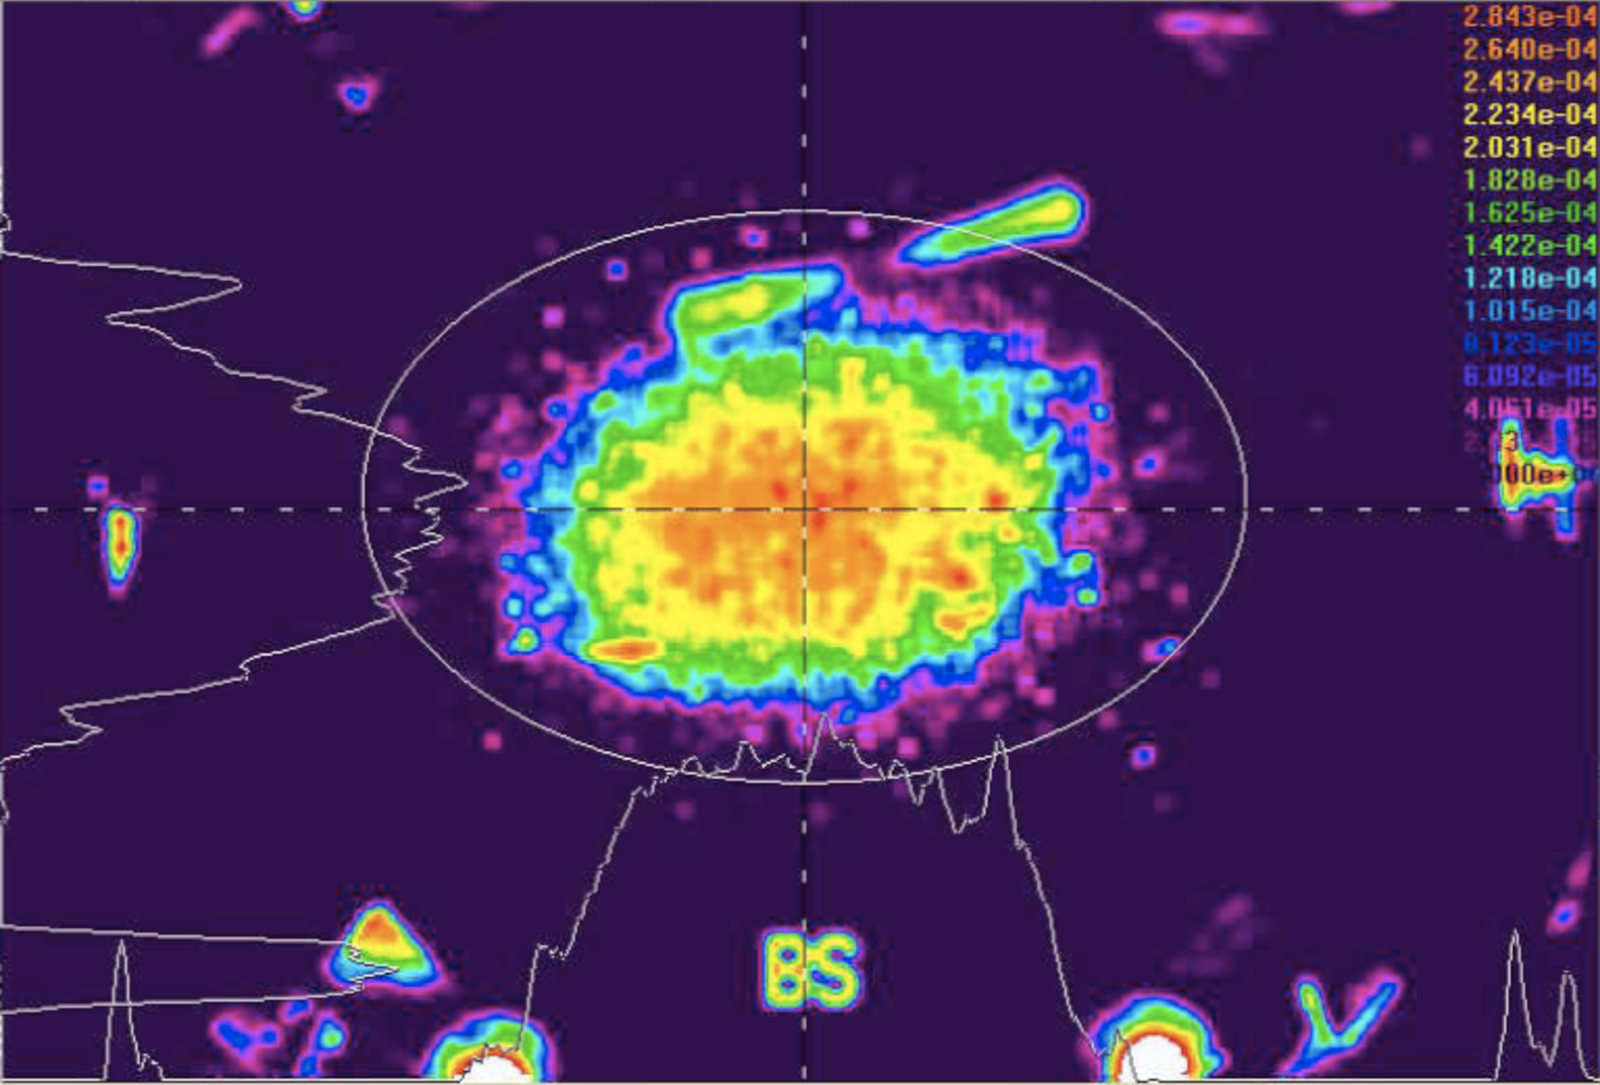
\includegraphics[width=0.8\textwidth]{figures/BCSspiricon.pdf}
% \caption{Image of beam on beam splitter as used for the beam centering servo.}
% \label{fig:BCS}
% \end{centering}
% \end{figure}


% \subsection{QPDs}  
% QPDX and QPDY see the small amount light that is transmitted through
% the ETMs, providing a monitor of the modal axes of the arm cavities. Together with the , they maintain the alignment of the input . QPDX 


% \subsection{WFSs}  
% The wavefront sensors provide the most sophisticated form of
% measuring angular motion of the mirrors. Their frame of reference is
% the fundamental Gaussian mode of the interferometer cavities (x-arm,
% y-arm, recycling cavity) as aligned to ???. All of the mirrors
% globally follow the pointing of the input beam (via the QPDs) which is
% in turn stabilized to the center of the beam splitter (via the BCS) at frequencies well
% below the pendulum resonances. The job of the wavefront sensors is to
% keep the mirrors aligned to one another up to several Hz within this
% hierarchy of alignment. The WFS provide DC and AC control to the
% mirror angles. 




% \section{Control}
% When the gain is really high, comparing the calibrated error and
% control signals shows just what the control loop is doing. The error
% is the residual and the control is what there would be without the
% loop.

% error * (1+G) is the motion without the loop, where G is the open loop gain.

% \begin{itemize} 
% \item optical lever calibration
% \item residuals, perhaps for different kinds of seismic
% \item compare to mirror motion with no ifo (demonstrate ASC suppression)
% \end{itemize}



\section{The Initial LIGO WFS basis}
In Initial LIGO, the basis for angular control was the sensor
basis. The wavefront sensors are located such that they sense
common/differential ETM/ITM angular motion. Thus, the filters were
designed to feedback to those sets of motions. This does not, however,
lend itself to easily handling radiation pressure torque. Since the
WFS basis is not the radiation pressure eigenbasis of Section
\ref{sec:eigenbasis}, each control servo must handle mixtures of the
soft and hard modes. Due to radiation pressure, each mirror has two
resonances, a more complicated plant than that offered by the
eigenbasis which has a single resonance for each mode. 

Since the soft mode is statically unstable, it needs high
(\textcolor{blue}{how high?}) DC gain at all times. In the WFS basis,
that would mean uniformly increasing the gains of all of the control
loops, since the control of the soft mode is split amongst the
loops. This poses a problem because increasing the gains impresses
sensing noise on the mirrors, affecting DARM, and impresses input beam
motion on the mirrors, making the interferometer as a whole less
steady. 

Once the Enhanced LIGO 35~W laser was installed and before
modifications to the Initial LIGO ASC basis were made, we succeeded in
operating the interferometer with 14~W input power. The unstable modes
were activated full force, but with high enough WSF gains, they were
controlled, albeit not that well. Figure ... shows a comparison of
DARM during the Nov 2008 lock in the old basis and an Enhanced LIGO
lock at the same power in the new basis. 



\section{Calibrations}
Since the data is collected digitally, the units are in digital
counts. This must be converted into physical units in order to make
meaningful statements beyond relative comparisons. Two ways to make a
calibration are to \textcolor{blue}{(think about this more!)}
\begin{itemize}
\item work backwards through the control system and electronics chain \vspace{-10pt}
\item inject an analog signal with a known amplitude 
\end{itemize}
I describe here the calibrations I made of some of the angular sensing
channels, all the while demonstrating particular examples of these
methods.


\subsection{Beam spot motion}
A quantity of interest is how much the beam moves on the ITMs and
ETMs. It is this beam spot motion which, together with the mirror
angular motion, creates a length signal that contributes noise to
DARM. An elegant way of following the motion of the beam on the test
masses is to track pickoffs of the light transmitted or reflected from
the mirrors. We have such signals naturally available for the ETMs and
ITMs from the QPDs which are otherwise used for ASC sensing. For
example, QPDX and QPDY see the light transmitted through each of the
ETMs and WFS2 sees the pickoff of light from the wedge of ITMX.

To calibrate the counts of the QPD and WFS2 pitch and yaw error
signals, \texttt{L1:ASC-QPDY\_\{PIT,YAW\}\_IN1} and
\texttt{L1:ASC-WFS2\_\{DCPitchMon, DCYawMon\}}, I moved the beam a
known distance on the test mass, $\Delta x$, and recorded the
corresponding $\Delta y$ of the QPD and WFS2 readback. The ratio
$\Delta x /\Delta y$ is the calibration from counts to meters. The
final calibrations of these channels are shown in Table
\ref{table:bsmcal} and the details of the procedure are described
below. \footnote{A minor technicality is that since there are no
  filters between the QPD error signals and the offset channel, their
  units are exactly the same. Thus, calculating meters of beam spot
  motion as a function of offset serves to calibrate the error
  point. For convenience, this is what I did.}

\begin{table}
\centering
\begin{tabular}{l l l l}
\hline
         & ETMX & ETMY & ITMs \\
\hline
pitch & 1.03e-5 m/ct & 1.21e-5 m/ct & 5.52e-2 m/ct \\
yaw & 0.88e-5 m/ct & 0.80e-5 m/ct & 4.79e-2 m/ct \\
\hline
\end{tabular}
\caption{Calibrations to be used with the QPDX, QPDY, and WFS2 DC
  pitch and yaw error signals for a measure of beam spot motion.}
\label{table:bsmcal}
\end{table}


\subsubsection{Moving the beam} 
Moving the beam on the mirrors is straightforward because of the ASC
system. All that we need to do is introduce an offset to the setpoint
of the of the beam centering aspect of the ASC servo. For the ETMs we
put a DC offset in the \texttt{L1:ASC-QPD\{X,Y\}\_\{PIT,
  YAW\}\_\{OFFSET\}} channel and for the ITMs we changed the $X$ and
$Y$ targets of the beam splitter beam centering servo.

\subsubsection{Measuring how much the beam has moved} 
The more difficult task is measuring just how much the beam has
moved. For this, we make use of the lever arm mechanism of angle to
length coupling. \textcolor{blue}{(This should be explained in the
  previous chapter, so maybe just reference it.)} The idea is that
when the axis of rotation of a mirror coincides with the center of the
beam, any tilt of the mirror about this axis does not affect the path
length of the reflected beam. However, if there is a mismatch between
rotation axis and beam location, then the light will pick up a
longitudinal phase shift when the mirror is tilted. During a full
interferometer lock, this is recorded by DARM.

The concept of the measurement is to move the axis of rotation of the
mirror so that it passes through the center of the beam. We use the
OSEMs to change the location of the axis of rotation, and we use DARM
to determine when the axis is aligned with the beam center. For
example, if we drive the top two osems more than the bottom two osems,
we've created an axis of rotation that sits below the center of
mass. The result of such tuning is an effective rebalance of the
center of mass of the mirror so that it is aligned with the center of
the beam. The procedure is:
\begin{enumerate}
\item Shake the mirror at some frequency $f$ (we use
39.5 Hz) during a full lock \vspace{-10pt}
\item Demodulate DARM at $f$ for several different sets of osem gains \vspace{-10pt}
\item Fit a quadratic to the demodulated data to pinpoint the osem gains that
  minimize the coupling to DARM
\end{enumerate}

Relating the osem gains to absolute beam position on the mirror
requires only the geometry of the mirror and osem setup. See
Fig. \ref{fig:mirror_osem_geometry}. We estimate the osem locations as
being on the edge of the mirror such that the length $d$ of one side
of the square that they form is given by $d =\sqrt{2} R$, where $R =
12.5$ cm is the radius of the mirror.  Then, collapsing the four osems
into a representative two at the centers of two opposite sides of the
square, we can evaluate where the pivot point is located relative to
center for a given force at each osem location. With the gain of each
OSEM given as $\pm (1 \pm \alpha)$ and setting the torques equal, we
have:
\begin{equation}
F [1+\alpha] x = F [1-\alpha][d-x].
\end{equation}
Therefore, the beam location relative to center is
\textcolor{blue}{(fix up notation)}
\begin{equation}
\Delta x := \frac{d}{2} - x = \alpha \frac{d}{2},
\end{equation}
and for a change in a pitch or yaw coil gain, the change in beam
position, $\Delta x$, is:
\begin{equation}
|\Delta{x}| = \frac{|\Delta{\mbox{gain}}| R}{\sqrt{2}} .
\end{equation}

\begin{figure}
\begin{centering}
%\includegraphics[width=1.0\columnwidth]{figures/}
\end{centering}
\caption{\textcolor{blue}{Place holder for mirror+osem geometry figure.}}
\label{fig:mirror_osem_geometry}
\end{figure}





\subsection{Angular mirror motion}


\begin{figure}
\begin{centering}
\includegraphics[width=1.0\columnwidth]{figures/OLcal_pitch.pdf}
\caption[Optical lever calibration]{Optical lever calibration data and fits to Eq. \ref{eq:pwr_disptilt} (pitch).}
\end{centering}
\end{figure}


\subsection{WFS error signals}



\section{Input beam motion}
\textcolor{blue}{Breakdown of source of mirror motion.}

The beam centering servo only operates up to about 10~mHz, meaning the
beam-centering degree of freedom is uncontrolled at higher
frequencies. The source of beam de-centering on the mirrors is input
beam motion. The HAM seismic isolation tables from which the input
optics are suspended have resonant ``stack'' modes from about 0.8~Hz
to 3~Hz. The excess table motion at these frequencies is transmitted
to the MMTs. 

I measured the impression of the input beam motion on the mirrors by
increasing the gain of the common-degree-of-freedom WFS servos (CH,
CS, RM) for about 10~minutes. Comparing the amount of angular
motion of the mirrors from this time of high common WFS gain to a time
with nominal WFS gain and similar seismic motion, we can see the
effect directly. Fig. \ref{fig:inputbeam_impression} shows comparison
spectra, demonstrating how there is higher test mass motion around
1~Hz when the common WFS gains are higher.

\begin{figure}
\begin{centering}
\subfigure{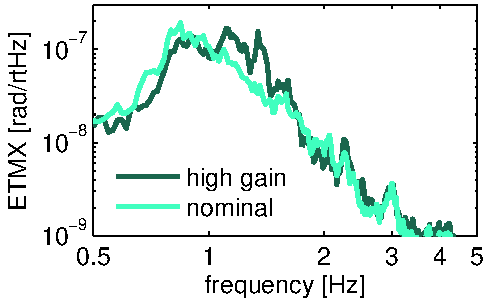
\includegraphics[width=0.333\textwidth]{figures/ETMX_highnom.pdf}}\subfigure{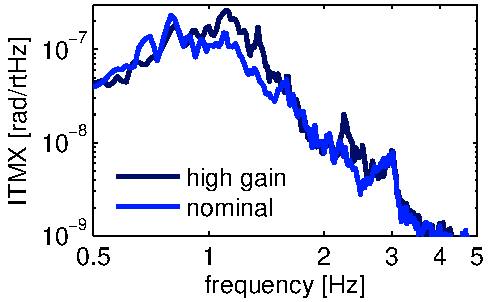
\includegraphics[width=0.333\textwidth]{figures/ITMX_highnom.pdf}}\subfigure{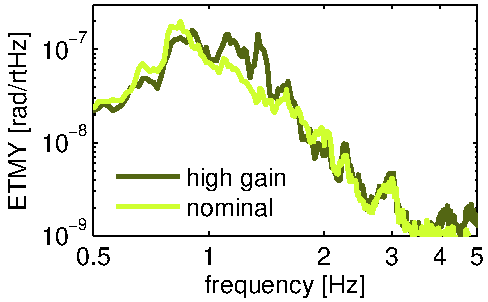
\includegraphics[width=0.333\textwidth]{figures/ETMY_highnom.pdf}}
\subfigure{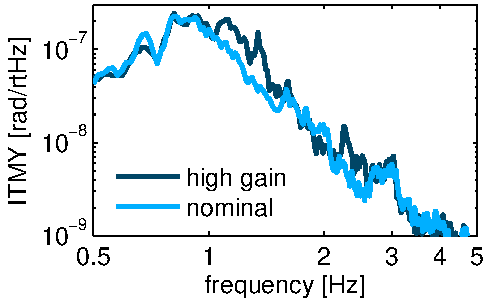
\includegraphics[width=0.333\textwidth]{figures/ITMY_highnom.pdf}}\subfigure{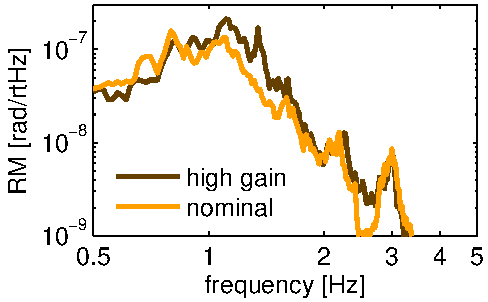
\includegraphics[width=0.333\textwidth]{figures/RM_highnom.pdf}}
\caption[Impression of input beam motion on the core mirrors]{Input beam motion impression on the core mirrors. Mirror
  motion when the common WFS gains (WFS2a, WFS3, WFS4) are increased by a
  factor of 2.5 is compared to mirror motion when the WFS gains are
  nominal. Both spectra come from a time of similar seismic activity
  (typical weekday afternoon noise).}
\label{fig:inputbeam_impression}
\end{centering}
\end{figure}

A more quantitative study of the effects of input beam motion is to
measure transfer coefficients between the input beam motion and the
mirror angular (or beam spot) motion. During a full interferometer
lock I put lines in MMT1, MMT2, and MMT3 at 1.05~Hz, 1.25~Hz, and
0.85~Hz, respectively, selecting excitation amplitudes large enough to
appear in the common WFS spectra. I compared the amplitudes of the
lines in the MMT spectra with those in the WFS spectra. The counts to
counts transfer coefficients are shown in Table
\ref{table:inputbeam_TFcoeffs}. Since sensing is flat, I use the shape
of the WFS loop to extrapolate this transfer coefficent at one
frequency to other frequencies. The result is a transfer function
useful for making a noisebudget of input beam motion to test mass
motion. Selecting a science mode time of typical day-time seismic
noise, I made a noisebudget as found in Fig. \ref{fig:inputbeam_NB}.

\begin{table}
\centering
\caption{\textcolor{blue}{Make this!!!}}
\begin{tabular}{l l l l l l}
\hline
\end{tabular}
\label{table:inputbeam_TFcoeffs}
\end{table}


\begin{figure}
\begin{centering}
%\includegraphics[width=1.0\columnwidth]{figures/}
\caption{\textcolor{blue}{Make this!!}}
\label{fig:inputbeam_NB}
\end{centering}
\end{figure}


\textcolor{blue}{Wiener filter beam spot motion to show corner seismic is primary
contributor when the WFS gains are high. Also show seismic noise 
coherent with mirror motion in general.}



\section{The marginally-stable Power Recycling Cavity}
The power recycling cavity (PRC) is the linear cavity formed by the RM
and ITMs. Since the radius of curvature of both the RM and the ITMs
points in the same direction, the cavity is geometrically
unstable. For example, in its cold state at LLO the $g$-factor of the
cavity is 1.00005 and at LHO it's 1.00003. The beam in the PRC is not
spatially contained and may be made of many higher order modes. The
heating of the ITMs from the kilowatts of power in the arm cavities
together with the ITM thermal compensation system (TCS) serve the role
of making the PRC geometrically stable for interferometer
operation. The heating and cooling of the ITMs is a very complicated
process and therefore not very precise, so the value of the hot PRC's
$g$-factor is usually not constant.

The changing $g$-factor has potentially severe consequences for the
ASC. Because of its geometry, the power build-up in the PRC is very
sensitve to both the mirror angles and the $g$-factor. Power
fluctuation is detrimental because the signal to noise ratios of the
sensors that probe the PRC light degrade due to the presence of
increased junk light that contributes shot noise but not
signal. WFS1Q, WFS2I, and WFS2Q are the most sensitive to the PRC
because their signals are derived from the 25~MHz sidebands. Their
sensitivity to mirror motion is therefore subject to change. Since
achieving a flat power build-up in the PRC is a difficult task (too
much motion in the PRC is quite often a cause of lock loss), we must
update the real-time control system to reflect their changing
sensitivites. Otherwise, the mirror angles will not be accurately
controlled.

An estimate of the expected power fluctuations based on the $g$-factor
and RM motion is a straightforward excercise when using
Eq. \ref{eq:cavitydisptilt_mirrorangle} and Eq. \ref{eq:pwr_disptilt}
as derived in the Appendix. If we estimate the $g$-factors of the RM
and ITM as $g_{RM} = 1+\delta$ and $g_{ITM} = 1 - \delta$ ($\delta =6
\times 10^{-4}$ for LLO the cold state) and approximate the distance
of each mirror to the cavity waist as $z$ since the two mirrors are
very close to each other compared to the waist location, then
Eq. \ref{eq:cavitydisptilt_mirrorangle} reduces to:
\begin{equation}
\left\llbracket \begin{array}{c}
a_{PRC} \\
\alpha_{PRC} \end{array} \right\rrbracket = 
\left\llbracket \begin{array}{cc}
z(2+\delta)/\delta & z(2-\delta)/\delta \\
-1/\delta & -1/\delta \end{array} \right\rrbracket
\left\llbracket \begin{array}{c}
\theta_{RM}\\
\theta_{ITM} \end{array} \right\rrbracket.
\end{equation}

Fig. \ref{fig:prc_power} plots the power in the PRC as a function of
$\theta_{RM}$ for several values of $\delta$, demonstrating
the sensitivity of the PRC to the ITM heating.  For example, the
typcial RM angular displacement of $10^{-7}$ rad results in a 66\%
power loss when the PRC $g$-factor is very near instability with a
value of $1-0.0001$. Only as the $g$-factor moves further from $1$
does the angular motion of the RM have less and less of an effect on
the power build-up.

\begin{figure}
\begin{centering}
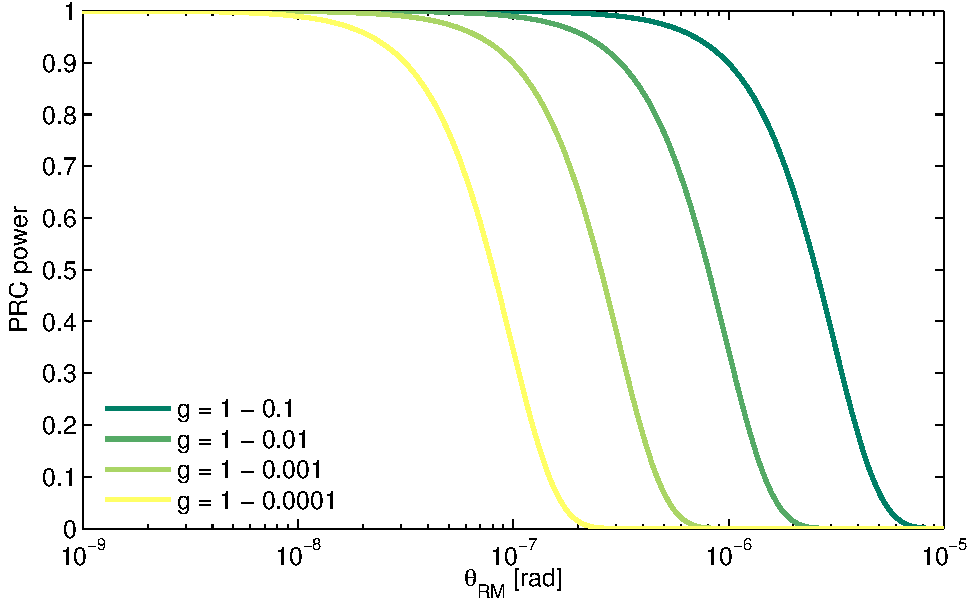
\includegraphics[width=1.0\columnwidth]{figures/prc_power.pdf}
\caption{Dependence of power build-up in the power recycling cavity on
  the PRC's $g$-factor and the RM tilt. TCS is necessary for
  stabilizing the PRC's geometry and therefore its sensitivity to
  mirror motion. For simplicity, the ITM is assumed stationary in
  these plots.}
\label{fig:prc_power}
\end{centering}
\end{figure}


\subsection{SPOB power scaling}
The effect of the marginally stable recycling cavity can be seen by
tracking the ASC sensing matrix elements as $g$ changes. I excited
three of the test masses (ETMX, ITMX, RM) at three different
frequencies (9.7~Hz, 10.7~Hz, and 11.7~Hz, respectively) during a full
interferometer lock and changed the TCS settings so that over the
course of 15 minutes the $g$-factor steadily changed. Demodulating
each of the WFS signals at each of the three excitation frequencies as
a function of time shows the strength of the WFS response to the motion
of these three mirrors over the course of the study. To compensate for
the difference in pendulum responses to the excitations, I multiplied
the demodulated signals for a particular excitation $f$ by
$(f/9.7)^2$. I also normalized the response by the phase of the
mirror's motion as witnessed by the optical levers.

The results are shown in Fig. \ref{fig:WFStrack}. As expected, WFS1Q,
WFS2I, and WFS2Q show dependence on the PRC power, and therefore the
$g$-factor. The WFS3 and WFS4 sensing elements are flat. The power in
the PRC as measured by the $2f$-demodulated POB signal, NSPOB,
is also shown in Fig. \ref{fig:WFStrack} for this time period. In
order to compensate for this $g$-factor dependence, we multiply the
WFS\{1Q, 2I, 2Q\} error signals in real-time by
\begin{equation}
\frac{1}{P_{in}} \left[\frac{NSPOB}{350}\right]^{-1/2}
\end{equation}
and WFS3I and WFS4I by $1/P_{in}$, where the 350 is the reference
NSPOB, treated as nominal. Thus, during interferometer operation, all
WFS signals are normalized to input power and are not dependent on the
PRC power. This correction to the WFS signals is called SPOB power
scaling.



\begin{figure}
\begin{centering}
\subfigure{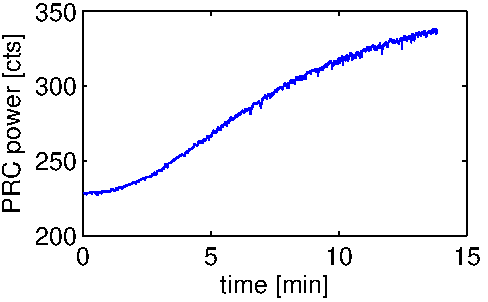
\includegraphics[width=0.5\textwidth]{figures/spob_gaintracking.pdf}}\subfigure{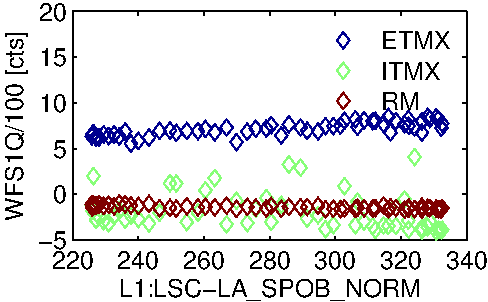
\includegraphics[width=0.5\textwidth]{figures/WFS1Q_track.pdf}}
\subfigure{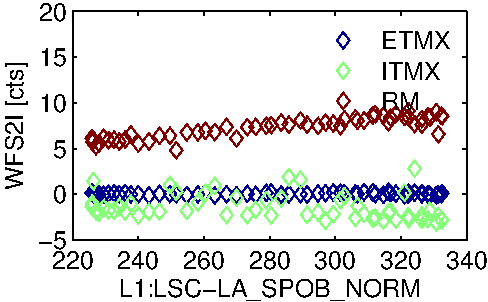
\includegraphics[width=0.5\textwidth]{figures/WFS2I_track.pdf}}\subfigure{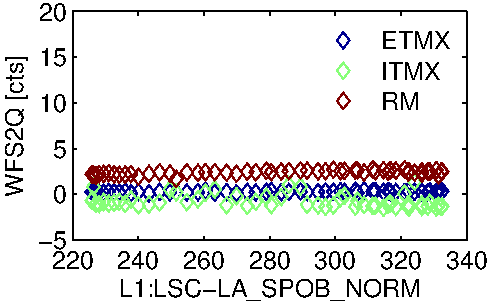
\includegraphics[width=0.5\textwidth]{figures/WFS2Q_track.pdf}}
\subfigure{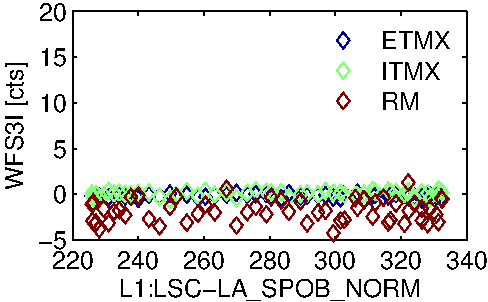
\includegraphics[width=0.5\textwidth]{figures/WFS3I_track.pdf}}\subfigure{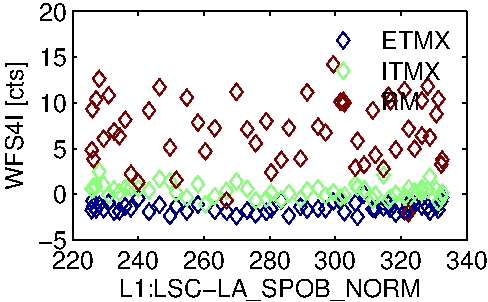
\includegraphics[width=0.5\textwidth]{figures/WFS4I_track.pdf}}
\caption{Measurement of the dependence of the WFS error signals on the
power recycling cavity geometry. WFS1Q, WFS2I, WFS2Q are more
sensitive to test mass motion as the power in the recycling cavity
increases. To achieve a dependable feedback system, the error signals
are scaled in real-time, forcing their responses to be flat with
power. This range of SPOB is low for normal operations.}
\label{fig:WFStrack}
\end{centering}
\end{figure}


\subsection{Sideband imbalance}
Show OSA scan of AS port.




\section{The ASC sensing matrix}



\subsection{Optical gain matrix}


\subsection{Diagonalizing the ASC drive matrix}




\section{DC readout related measurements}
\begin{itemize}
\item RF created from DC offset beam moving on WFS1
\item RF vs DC vs power comparison of (AS) beam spot motion on WFS1
\end{itemize}


% \section{ASC noisebudget}
% \begin{itemize}
% \item seismic - breakdown of soure of motion
% \item L2A
% \item input beam 
% \item electronics noise
% \item shot noise
% \end{itemize}




\section{The effect of the ASC}


\begin{figure}
\begin{centering}
%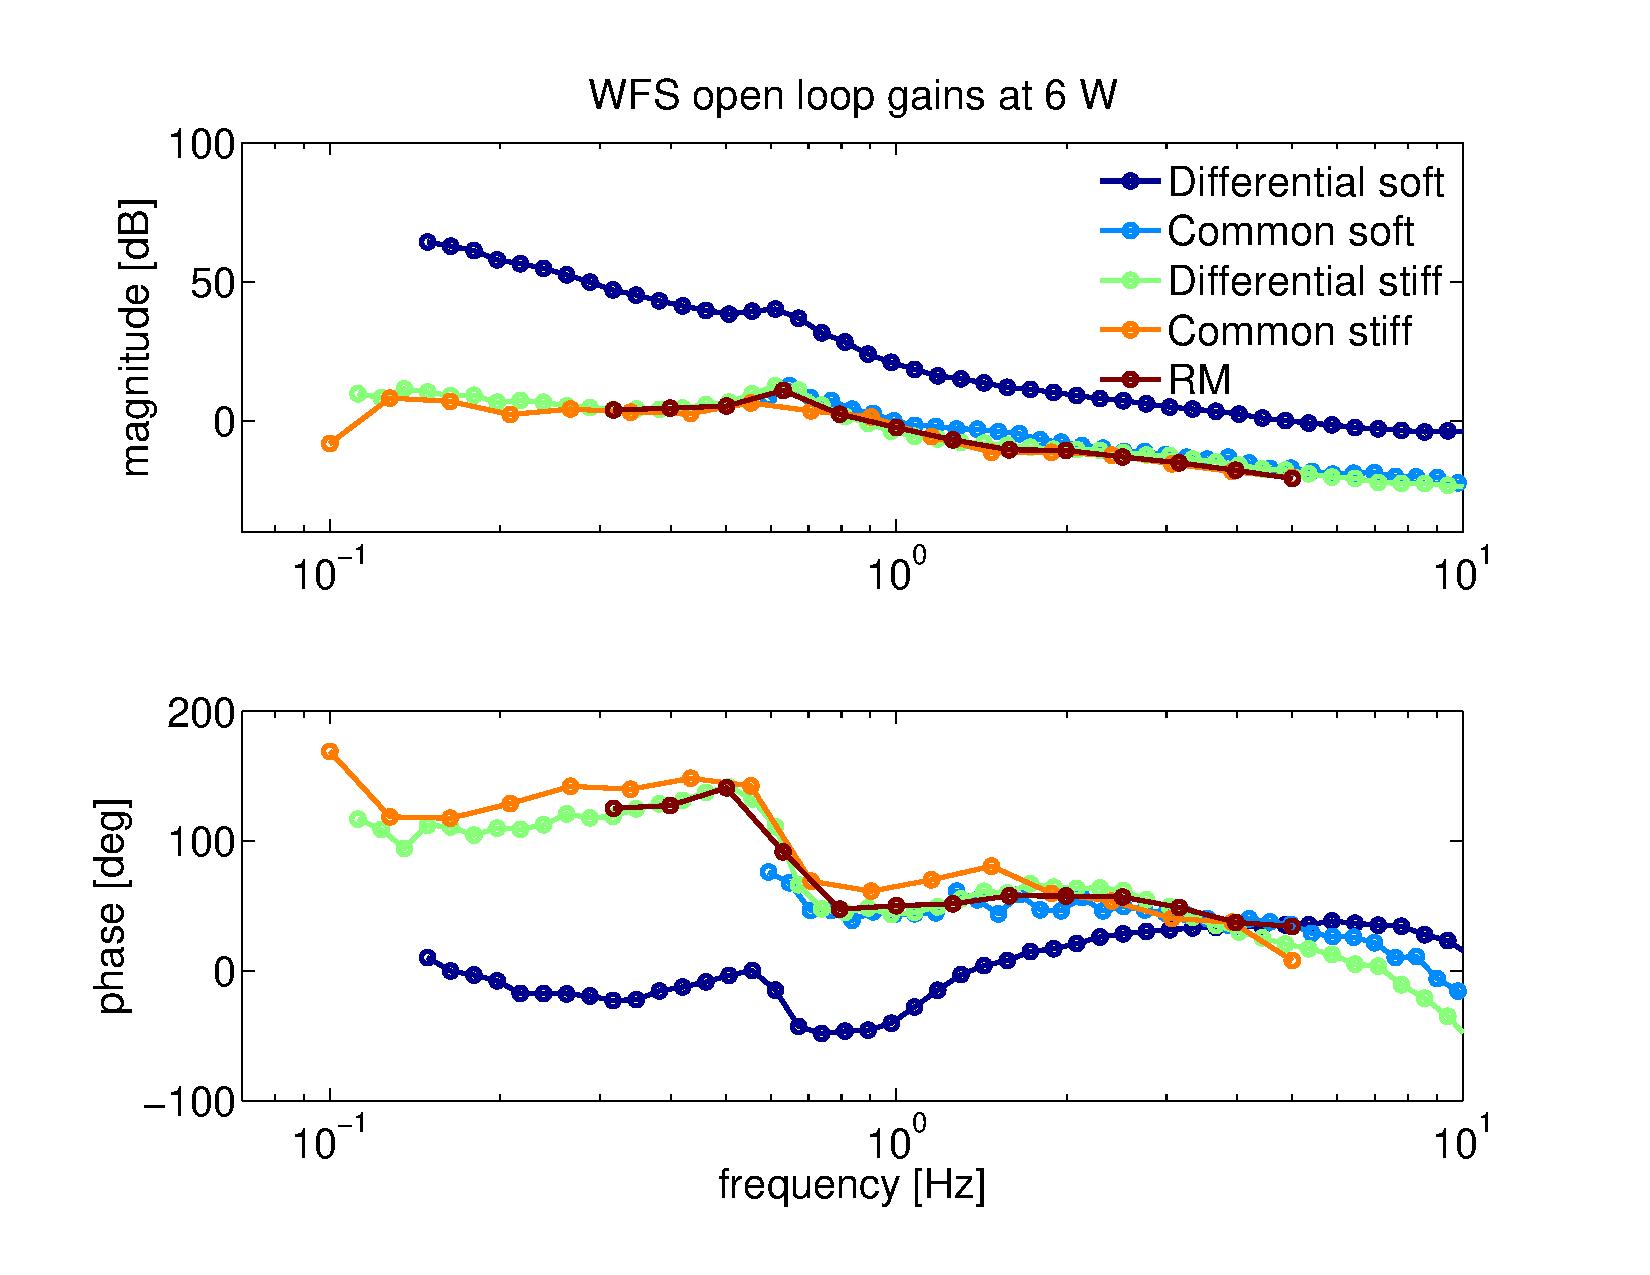
\includegraphics[width=0.8\columnwidth]{figures/olgs6W.pdf}
\subfigure{\includegraphics[width=1.0\columnwidth]{figures/allolgs_6W_mags.pdf}}
\subfigure{\includegraphics[width=1.0\columnwidth]{figures/allolgs_6W_phases.pdf}}
\caption{Open loop gains (pitch) of the 5 WFS loops as measured with 6 W
  input power.}
\label{fig:olgs6W}
\end{centering}
\end{figure}


\begin{figure}
\begin{centering}
\subfigure{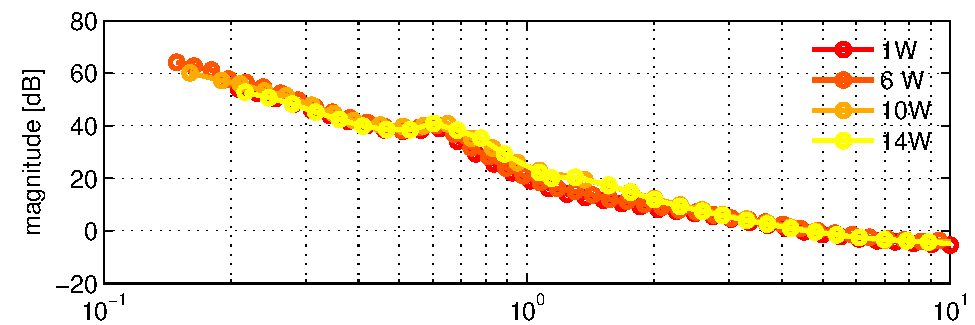
\includegraphics[width=1.0\columnwidth]{figures/wfs1_olgs_mags.pdf}}
\subfigure{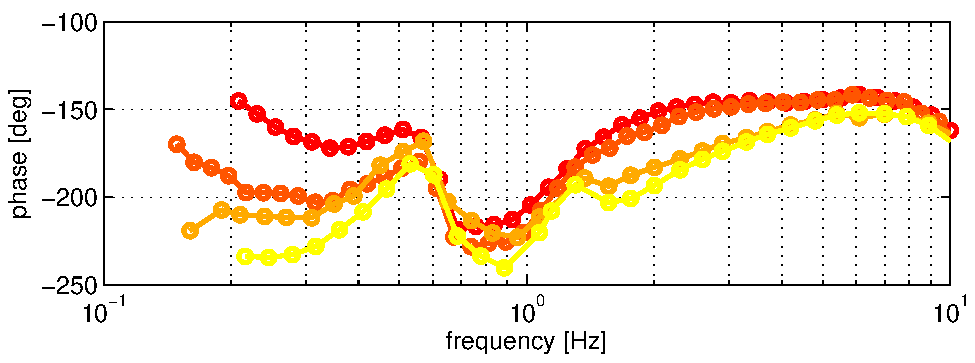
\includegraphics[width=1.0\columnwidth]{figures/wfs1_olgs_phases.pdf}}
\caption{Open loop gains (pitch) of the differential soft (WFS1) loop as measured at four
  different powers.}
\label{fig:DSolgs}
\end{centering}
\end{figure}

\begin{figure}
\begin{centering}
\subfigure{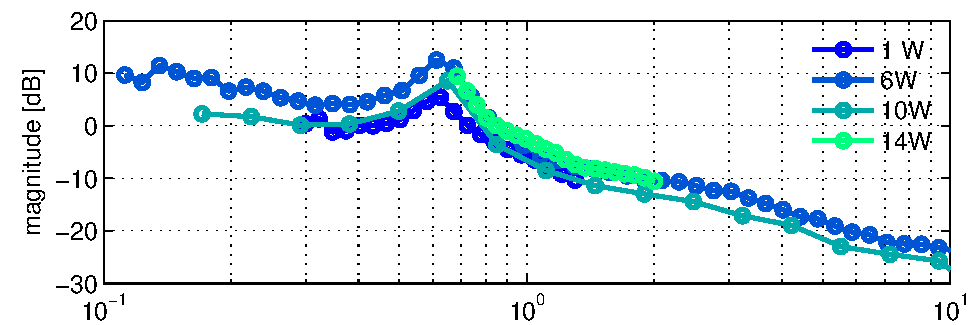
\includegraphics[width=1.0\columnwidth]{figures/wfs2b_olgs_mags.pdf}}
\subfigure{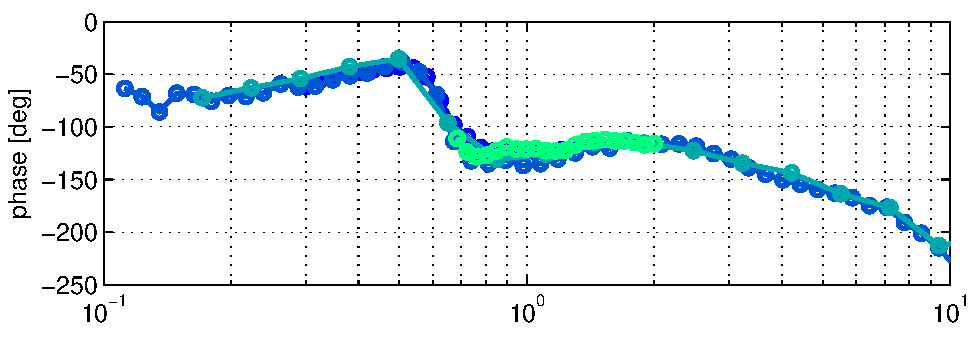
\includegraphics[width=1.0\columnwidth]{figures/wfs2b_olgs_phases.pdf}}
\caption{Open loop gains (pitch) of the differential hard (WFS2B) loop as measured at four
  different powers.}
\label{fig:DHolgs}
\end{centering}
\end{figure}

\begin{figure}
\begin{centering}
\subfigure{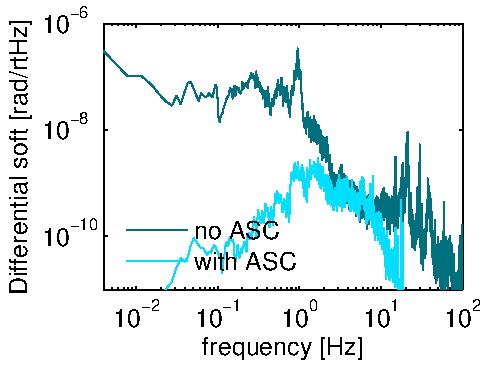
\includegraphics[width=0.5\textwidth]{figures/onoff_DS.pdf}}\subfigure{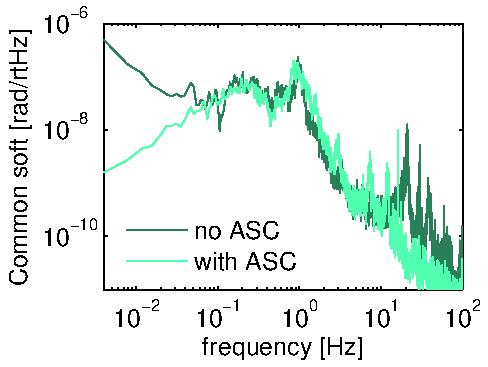
\includegraphics[width=0.5\textwidth]{figures/onoff_CS.pdf}}
\subfigure{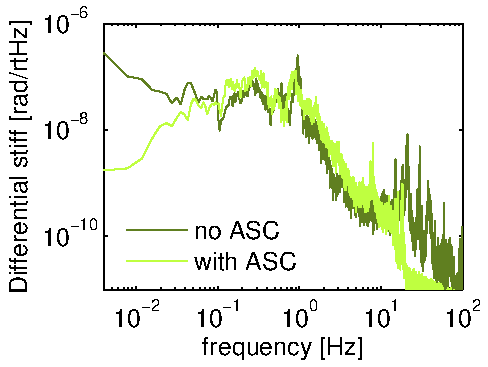
\includegraphics[width=0.5\textwidth]{figures/onoff_DH.pdf}}\subfigure{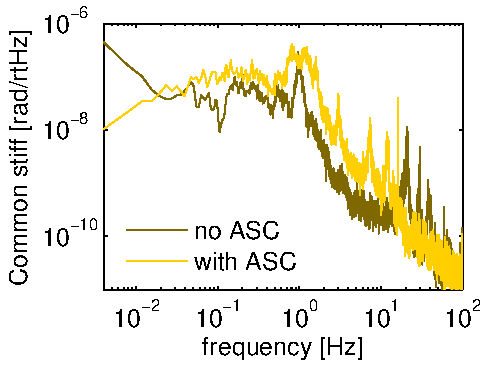
\includegraphics[width=0.5\textwidth]{figures/onoff_CH.pdf}}
\subfigure{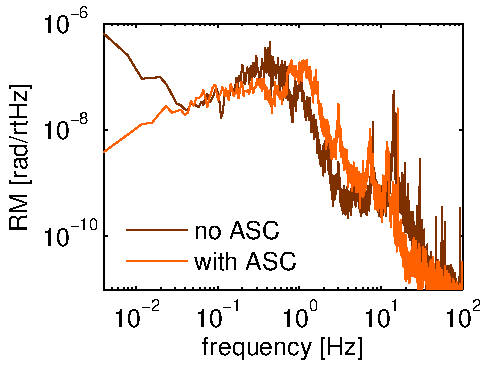
\includegraphics[width=0.5\textwidth]{figures/onoff_RM.pdf}}
\caption{Propagation of sensor signals from 10 W lock through
  input matrix and power scaling to eigenbasis, compared with
  eigenbasis reconstruction of optical lever signals when
  interferometer not locked, but optics under oplev damping. Data are
  taken 45 minutes apart. \textcolor{blue}{Perhaps include loop-undone
  backgrounds, too, using my measured OLTFs. FIX POWER SCALING.}}
\label{fig:}
\end{centering}
\end{figure}


% \begin{figure}
% \begin{centering}
% 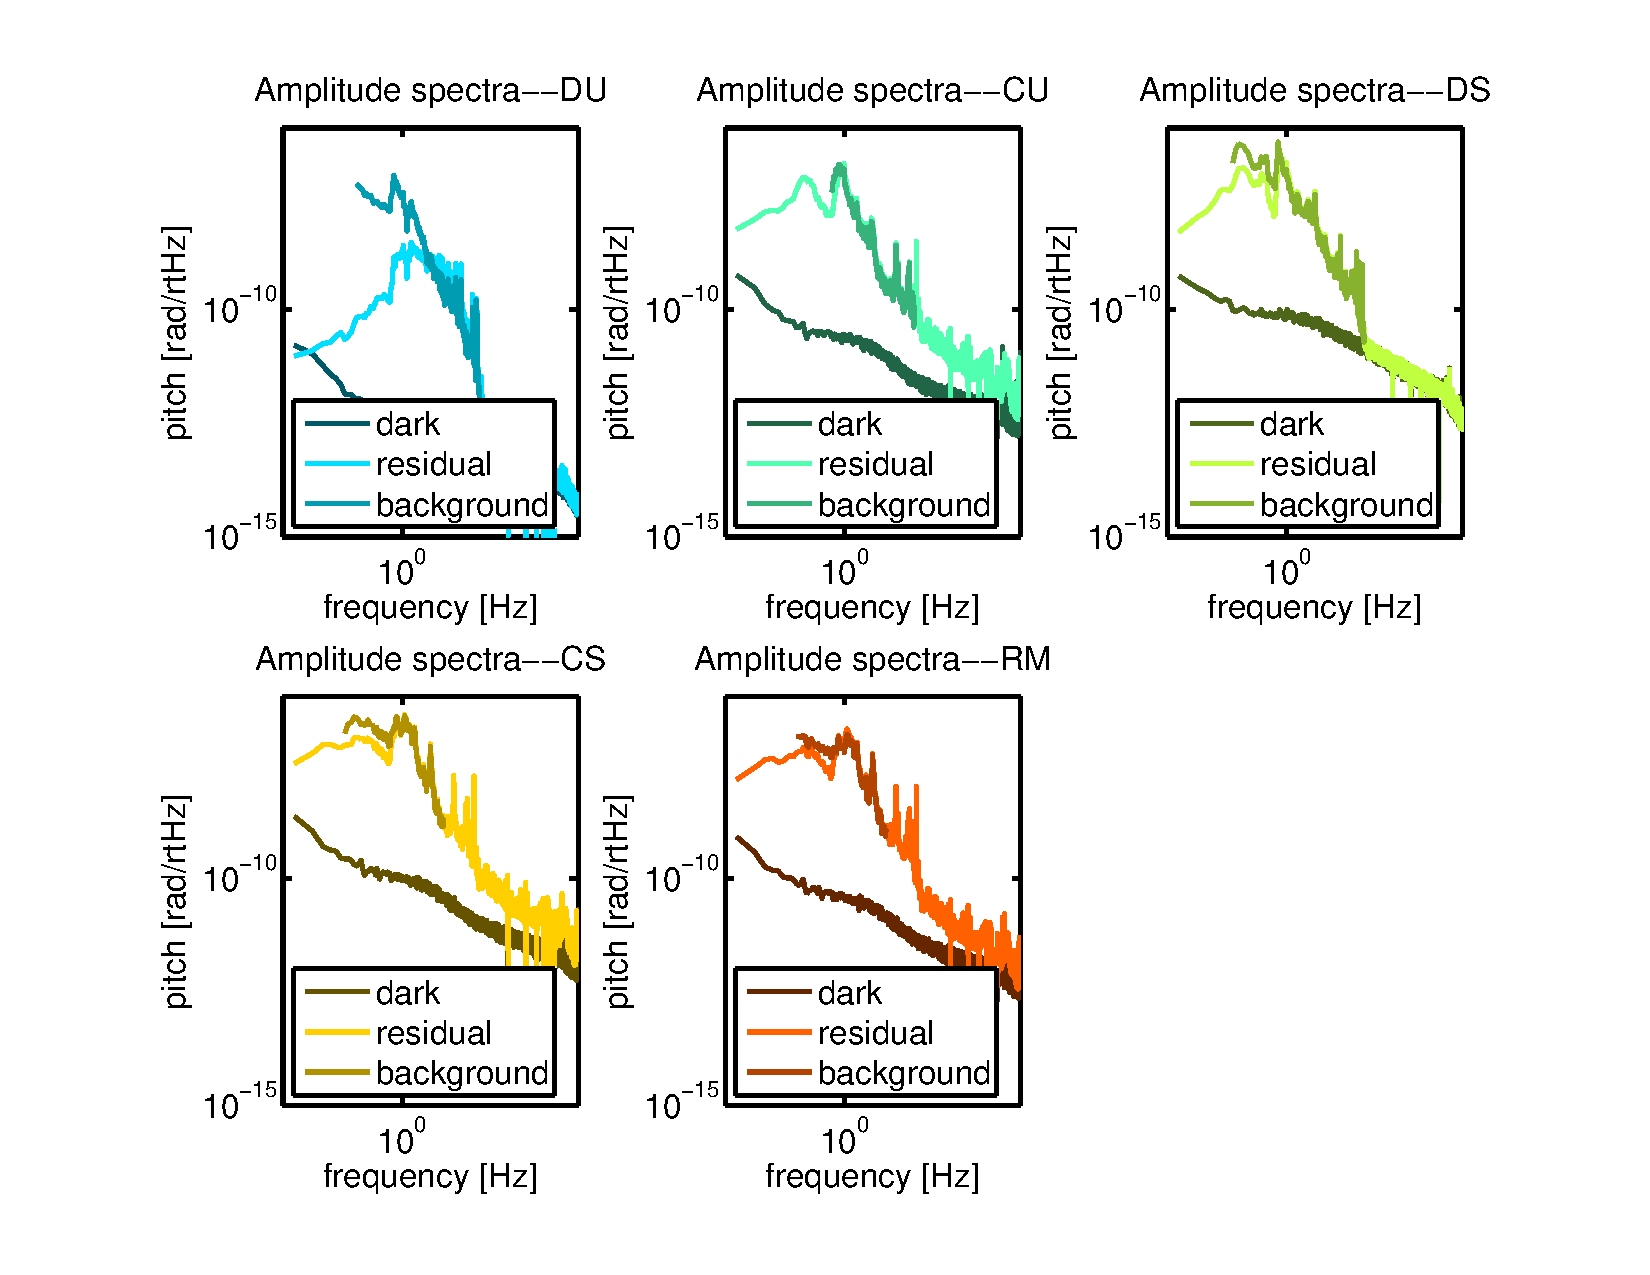
\includegraphics[width=0.7\textwidth]{figures/ASCdofsignals.pdf}
% \caption{Top: Comparison of motion with and without the
%   ASC. Eigenbasis residual during 10 W lock, and background derived
%   from loop correction. Completely different day from next
%   plot. (Perhaps merge with next plot)}
% \label{fig:}
% \end{centering}
% \end{figure}




\section{ASC to DARM noisebudget}
Broadband effect on DARM.

\subsection{Tuning the cut-off filters} 
The cut-off frequency of the lowpass filters for the WFS control are
of particular importance in the DARM noisebudget. The lowpass filter
is necessary for suppressing the impression of sensing noise on
suspension control. 

\begin{figure}
\begin{centering}
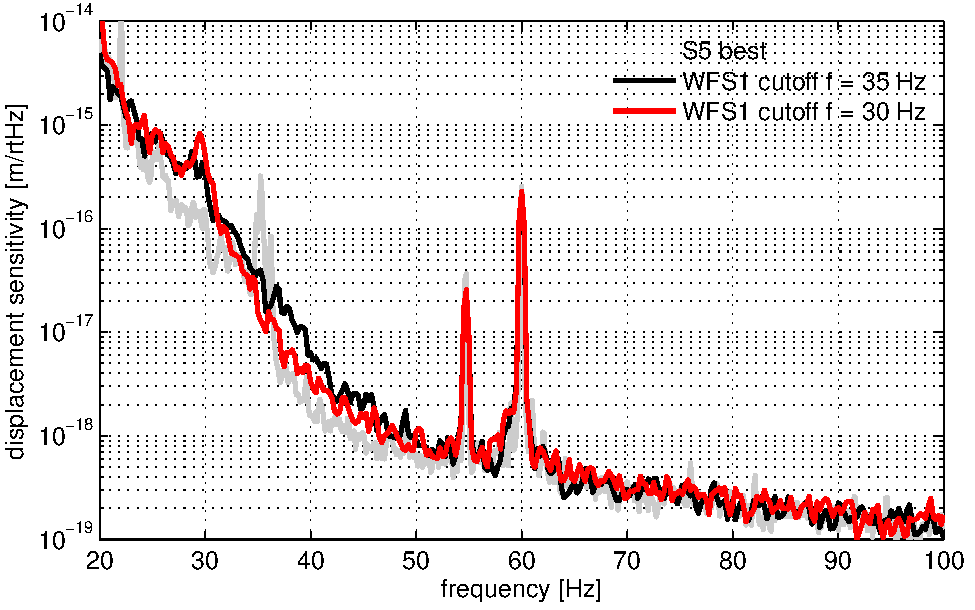
\includegraphics[width=1.0\textwidth]{figures/cutoffWFS1_DARMcompare.pdf}
\caption{Effect of the WFS1 lowpass filter cutoff frequency on strain sensitivity.}
\label{fig:WFS1cutoff}
\end{centering}
\end{figure}




\begin{figure}
\begin{centering}
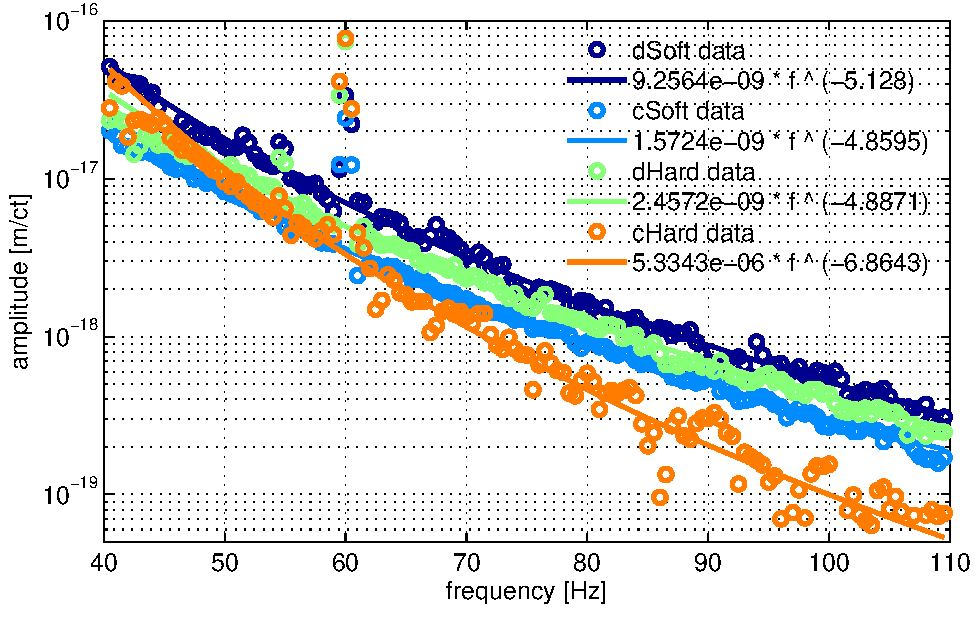
\includegraphics[width=1.0\columnwidth]{figures/ASC2DARM_TFs.pdf}
\caption{ASC to DARM transfer function for four of the five wavefront
  sensor loops. The RM to DARM transfer function could not be measured
  because the contribution is so small. The fitted curves can be
  multiplied by the WFS error signals at any time to calculate the ASC
  noise contribution to DARM. \textcolor{blue}{Need to turn cts into Watts.}}
\end{centering}
\end{figure}




\section{Feed-forward}


\section{Advanced LIGO}
The Advanced LIGO interferometers will have heavier mirrors, a stable
recycling cavity, and more circulating power. 